\section{Middleware Design}
\label{sec:design}

Our middleware framework mainly consists of two layers: event definition language (EDL) and event detection framework. The overall architecture of PSWare is shown in Figure \ref{fig:psware-architecture}.

\begin{figure}
\centering
\subfloat[System architecture]{\label{fig:psware-architecture}\figurehalfwidth{psware-architecture}}
\subfloat[EDL compiler structure]{\label{fig:edlcompiler}\figurehalfwidth{edlcompiler}}
\caption{PSWare design}
\label{fig:psware-design}
\end{figure}

To use the middleware, applications developers will first define event types according to the application requirements. Then the subscription may be defined by specifying the constraints and relations of the predefined event types. The subscription will then be compiled and processed by the EDL compiler and be disseminated into the network. When the events are detected by the sensor nodes, they will be delivered to the application.

\subsection{EDL and Its Compiler}
PSWare is type-based \cite{facespubsub} pub/sub system since it is easier to define composite events by specifying the event types. Our subscription contains one or more event declaration and one subscribing statement. The subscribe statement simply uses the keyword 'subscribe' followed the event type name needed by the application. Each event type declaration can have up to three parts: the event body, the where clause and the on clause. The event body defines the attributes of the events. The on clause are used to specify the sub-events used by a composite event. The where clause defines the filter of the corresponding event type.

The on clause and the where clause are both optional in case if the event is primitive or doesn't have a filter. The syntax of the on clause is almost exactly the same as the field declaration so it is not repeatedly listed. The key difference between the two is that the on clause lists sub-events instead of fields. The two are separated for a clear code presentation and easier type checking. The where clause simply consists of conditional expressions so that the filters may be defined by specifying the operators.

A simple example of using EDL is shown in Listing \ref{prog:originaledl}. In this example, two events, 'SimpleEvent' and 'CompEvent' are defined. 'SimpleEvent' is a primitive event which occurs when the detected temperature reading is above certain threshold. 'CompEvent' is a composite event that is based on two events of 'SimpleEvent' and their time must satisfy a certain condition in order to indicate the occurrence of 'CompEvent'.
\begin{lstlisting}[caption=A simple EDL program, label=prog:originaledl]
Event SimpleEvent {
	int temp=System.temp;
	int id=System.id;
	int time=System.time;
} where {
	temp > 30
}
Event CompEvent {
} on {
	SimpleEvent e1 and
	SimpleEvent e2
} where {
	e2.time-e1.time=600
}
\end{lstlisting}

The EDL-based subscription will be processed by our EDL compiler. The output of the compiler has two parts as shown in Figure \ref{fig:edlcompiler}. The first part is the byte codes which will be executed by individual sensors to detect events. We will discuss how the sensor nodes will execute the byte codes in the next section. The second part is the event receiving module. This module is responsible for receiving and interpreting the events delivered from WSN and notify the application layer if the subscribed events are delivered.

\begin{figure}
\centering
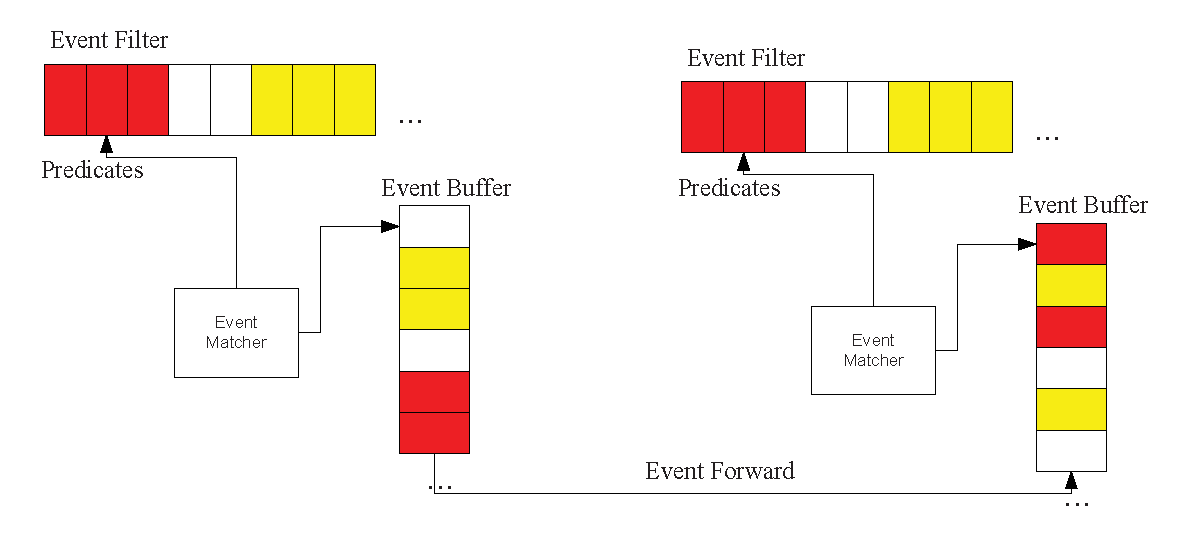
\includegraphics[width=.8\textwidth]{eventdetectionframework2}
\caption{Event detection framework}
\label{fig:eventdetectionframework2}
\end{figure}

\subsection{Runtime Event Detection Framework}
The byte codes generated by the compiler can be further divided into three parts: event meta data, event filters and event matcher. Event meta data contains the description of the event types such as event type ID, event size and the types of attributes for each event. Event filters are the constraints defined for each event type. Event matcher schedules the execution for event detection according to the subscription and event relations.

The event filters use an idea that is similar to the VM-based approach \cite{mate} in the sense that the filters are broken down into some basic operations called instructions. Such design choice is for the extensibility of the middleware so that different event filters and detection mechanisms may be easily implemented through the operations. There are mainly three types of instructions used by PSWare:
\begin{itemize}
\item Stack instructions: PSWare uses a vector-based architecture so that the operands are implicitly specified on the stack. Such design can allow compact code size. Instructions falling into this category includes pop, push and copy.
\item Mathematical instructions: these instructions are used to implement the necessary operators used in the filters. They can be further divided into four sub-categories including basic mathematical instructions (e.g. addition, subtraction, multiplication, division), logical instructions (e.g. logical and, logical or), relational instructions (e.g. greater than, less than, eqal) and bitwise instructions (e.g. shift).
\item Event instructions: these are the instructions related to event detection. We will discuss about them in more details in the latter part of the section.
\end{itemize}

\begin{comment}
In addition to the filters, as shown in Figure \ref{fig:pswarevm}, each sensor node has an event buffer where the detected events may be stored for composite event detection.

\begin{figure}
\centering
\figurecurrentwidth{pswarevm}
\caption{PSWare runtime environment}
\label{fig:pswarevm}
\end{figure}
\end{comment}

The essential operations for our event detection framework is shown in Figure \ref{fig:eventdetectionframework2}. In this framework, the event matcher will first fetch the events from the event buffer and then evaluate them against the corresponding filters. If the event has been detected, then it will be transmitted over the network based on certain event detection algorithms so that higher level composite events may be detected.

\subsection{Customization for Event Detection}
There are mainly three instructions related to event processing in PSWare:
\begin{itemize}
\item Create: when the event matcher begins to evaluate an event type, it will first create a temporary event and then evaluate it against its filter. This instruction is used to create such a temporary event.
\item Fetch: whenever an event of type \(e\) is being evaluated, this instruction is invoked to fetch such an event from the event buffer.
\item Evaluate: when an event is detected to occur, this instruction is used to take corresponding actions.
\end{itemize}

The event detection framework of PSWare is developed using NesC \cite{nesc}. In order to implement different event detection algorithms, one may re-implement the above three instructions if necessary with the APIs provided by PSWare. Due to the page limit, we omitted our discussion on PSWare's APIs and how to make use of them.